\documentclass[tikz]{standalone}

\usepackage{tikz}
\usepackage{tcolorbox}
\usepackage{pagecolor}
\usepackage{amsmath}
\usepackage{color}
\usepackage{blkarray}
\usepackage{graphicx}

\definecolor{mygray}{gray}{0.7}
\pagecolor{white}


\begin{document}
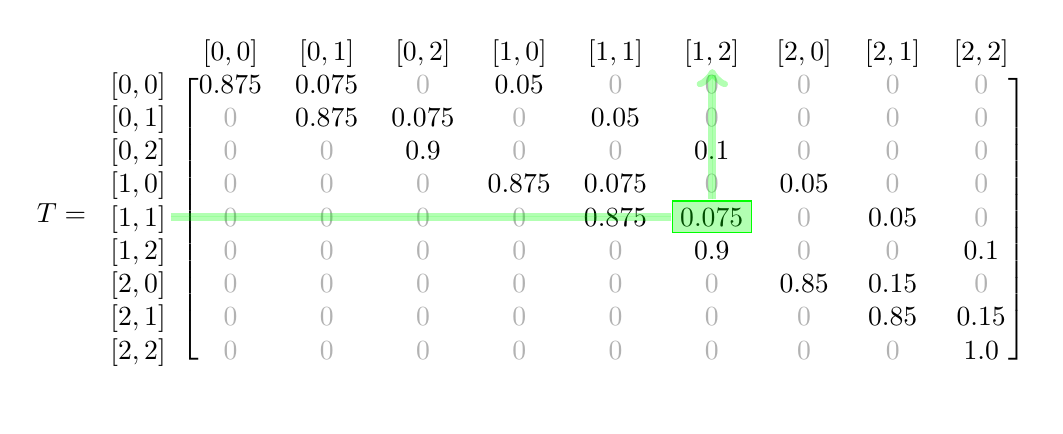
\begin{tikzpicture}

\node (A) at (-4.7, 0) {};
\node (B) at (1.9, 0) {};
\node (C) at (2.3, .1) {};
\node (D) at (2.3, 2 ) {};
\node (E) at (2.8, 0.2) {};
\node (F) at (1.8, -0.2) {};


\node (0) [] at (0, 0) {$T=
\begin{blockarray}{cccccccccc}
& [0, 0] & [0, 1] & [0, 2] & [1, 0] & [1, 1] & [1, 2] & [2, 0] & [2, 1] & [2, 2] \\
\begin{block}{c[ccccccccc]}
    {[0,0]} & 0.875 & 0.075 & \textcolor{mygray}{0}& 0.05 & \textcolor{mygray}{0}& \textcolor{mygray}{0}& \textcolor{mygray}{0}& \textcolor{mygray}{0}& \textcolor{mygray}{0}\\
    {[0,1]} & \textcolor{mygray}{0}& 0.875 & 0.075 & \textcolor{mygray}{0}& 0.05 & \textcolor{mygray}{0}& \textcolor{mygray}{0}& \textcolor{mygray}{0}& \textcolor{mygray}{0}\\
    {[0,2]} & \textcolor{mygray}{0}& \textcolor{mygray}{0}& 0.9 & \textcolor{mygray}{0}& \textcolor{mygray}{0}& 0.1 & \textcolor{mygray}{0}& \textcolor{mygray}{0}& \textcolor{mygray}{0}\\
    {[1,0]} & \textcolor{mygray}{0}& \textcolor{mygray}{0}& \textcolor{mygray}{0}& 0.875 & 0.075 & \textcolor{mygray}{0}& 0.05 & \textcolor{mygray}{0}& \textcolor{mygray}{0}\\
    {[1,1]} & \textcolor{mygray}{0}& \textcolor{mygray}{0}& \textcolor{mygray}{0}& \textcolor{mygray}{0}& 0.875 & 0.075 & \textcolor{mygray}{0}& 0.05 & \textcolor{mygray}{0}\\
    {[1,2]} & \textcolor{mygray}{0}& \textcolor{mygray}{0}& \textcolor{mygray}{0}& \textcolor{mygray}{0}& \textcolor{mygray}{0}& 0.9 & \textcolor{mygray}{0}& \textcolor{mygray}{0}& 0.1 \\
    {[2,0]} & \textcolor{mygray}{0}& \textcolor{mygray}{0}& \textcolor{mygray}{0}& \textcolor{mygray}{0}& \textcolor{mygray}{0}& \textcolor{mygray}{0}& 0.85 & 0.15 & \textcolor{mygray}{0}\\
    {[2,1]} & \textcolor{mygray}{0}& \textcolor{mygray}{0}& \textcolor{mygray}{0}& \textcolor{mygray}{0}& \textcolor{mygray}{0}& \textcolor{mygray}{0}& \textcolor{mygray}{0}& 0.85 & 0.15 \\
    {[2,2]} & \textcolor{mygray}{0}& \textcolor{mygray}{0}& \textcolor{mygray}{0}& \textcolor{mygray}{0}& \textcolor{mygray}{0}& \textcolor{mygray}{0}& \textcolor{mygray}{0}& \textcolor{mygray}{0}& 1.0\\
\end{block}
\end{blockarray}
$};

\draw [->,
    line width=1mm,
    draw=green,
    fill=green,
    draw opacity=.3]
    (A) -- (B) (C) -- (D);

\draw[fill=green, fill opacity = .3, draw=green] (E) rectangle (F);


\end{tikzpicture}
\end{document}
